\chapter{Methane hydrates}
\label{ch:state_of_the_science}
Gas hydrates are clathrate compounds, which means they consist of host molecules forming a lattice that traps guest molecules. Special to clathrate \emph{hydrates}, which are clathrates where water form the lattice, is that the structure is stabilized by the guests, and would collapse into regular ice or liquid water without guests present. Methane hydrates are among the more prevalent clathrate hydrates, and are formed by water molecules providing cages that host methane molecules. The most common cage structures are comprised of pentagonal and hexagonal faces forming regular cage structures. These structures can be described as replications of relatively simple unit cells. This work focus on methane hydrates, but since other clathrate hydrates have also been researched, and are relevant, they will be mentioned.

\section{History, occurrence and resource potential}
Gas hydrates were probably discovered as early as in the late 1700's by Sir Joseph Priestly, and the definitive confirmation of their existence was done by Sir Humphry Davy in 1810 \cite{Hester2009}. Early studies focused on identifying possible guest molecules in gas hydrates, but when methane-containing hydrates were shown to form in pipelines in 1934 \cite{Hammerschmidt1934}, \emph{methane} hydrates got more attention. However, the discovery of methane hydrates occurring in natural deposits was not made until the 1960's \cite{Makogon200714}. Methane hydrates are now known to occur in mud, sand, permafrost and on the sea floor around the world, within what is called the \emph{gas hydrate stability zone} (GHSZ). The GHSZ is characterized by low temperatures and high pressures compared to the stability zone of pure water ice. Figures \ref{fig:stability_permafrost} and \ref{fig:stability_seawater} illustrate the stability zones in permafrost and under the sea floor, respectively. Special to the sea-floor conditions is that the deeper the water, the deeper the stability zone beneath the sea floor, since sea floor temperature is almost constant. The stability zone for methane hydrate starts at around \SI{300}{\meter} in seawater and \SI{100}{\meter} in permafrost \cite{Hester2009}. In order for methane hydrates to actually occur, methane is needed. The methane is supplied either from biogenic or thermogenic methane sources. The geological setting of the hydrate formation is illustrated in figure \ref{fig:geological_setting} According to the World Ocean Review \cite{Bucker2014}, methane hydrates are mainly found on the continental slopes and in arctic permafrost.  Since methane hydrates reserves were discovered, estimates of total reserves have mainly been done for hydrates in marine sediments. The estimates have varied greatly, but the overall tendency has been a decline in the estimated amounts. Early estimates were as high as \SI{10000}{\giga\tonne} of carbon, but it has later been argued that the an amount of 500–\SI{2500}{\giga\tonne} is more reasonable \cite{Milkov2004183}. A fairly recent study by \citet{Wallmann2012} estimates the global reserves of carbon in methane hydrates in marine sediments to more than \SI{455}{\giga\tonne}. This estimate comes with a geographical distribution of the reserves, which is shown in figure \ref{fig:hydrate_map}. This estimate is much smaller than the early estimates, but it is still large compared to the \emph{proven} natural gas reserves in the world, which is roughly \SI{120}{\giga\tonne} (2013, \cite{CIA2013}) of carbon. It must further be assumed that only a fraction of these resources are recoverable, but these numbers still leave the possibility of methane hydrates playing an important role in the world energy mix. Some countries, like Japan and India, are very coal-dependent and seek to diversify their energy mix. If methane hydrates turn out to be viable, they can be of great economic importance to such countries. 


\begin{figure}
\centering
\begin{tikzpicture}
\draw[very thick,->] (0,6) -- (8,6) node[midway, above] (temptext) {Temperature};
\draw[very thick,->] (0,6) -- (0,0) node[midway, above, rotate=90] (depthtext) {Depth (pressure)};
\draw[step=1cm,gray,very thin] (0,0) grid (8,6);
\foreach \x in {0,1,2,3,4, 5, 6}
    \draw (\x cm,1pt) -- (\x cm,-1pt) node[anchor=north] {};
\foreach \y in {0,1,2,3,4, 5, 6}
    \draw (1pt,\y cm) -- (-1pt,\y cm) node[anchor=east] {};
\draw[name path=stability] (0, 4.5) .. controls (3.0, 4.5) and (4, 3.5) .. (4, 0); % Stability
\draw[name path=geoterm] (0, 6) -- (2, 3.0) -- (6, 0); % Geoterm parmafrost
\draw[dashed] (0, 3) -- (8, 3) node[above, xshift=-1.7cm] (textpermafrost) {Base of permafrost};
\fill[blue!40!white!]
	(0, 4.5) .. controls (3.0, 4.5) and (4, 3.5) .. (4, 0) -- (0, 0) -- (0, 4.5);
\draw[name path=stability, very thick, postaction={decorate, decoration={text along path, text align=center, raise=2pt, text={Hydrate phase boundary}}}] (0, 4.5) .. controls (3.0, 4.5) and (4, 3.5) .. (4, 0); % Stability
\draw[red, name path=geoterm, very thick, postaction={decorate, decoration={text along path, text align=left, raise=-10pt, text={Geotherm.}}}](2, 3.0) -- (6, 0); % Geoterm parmafrost
\draw[red, very thick] (0, 6) -- (2, 3.0);
\draw[dashed, very thick, blue] (0, 4.45) -- (8, 4.45);
\draw[dashed, very thick, blue] (0, 1.55) -- (8, 1.55);
\draw [decorate,decoration={brace,amplitude=10pt,mirror,raise=4pt},yshift=0pt]
(8 ,1.55) -- (8, 4.45) node [black,midway,xshift=0.8cm, rotate=90] {GHSZ};
\end{tikzpicture}
\caption{Gas hydrate stability conditions in permafrost (blue filled area). The red line shows the temperature as a function of deptth. In permafrost, the temperature is always increasing with increasing depth. This leaves a limited depth zone where the temperature–pressure configuration id within the gas hydrate stability conditions. This is the gas hydrate stability zone (GHSZ).}
\label{fig:stability_permafrost}
\end{figure}

\begin{figure}
\centering
\begin{tikzpicture}
\draw[very thick,->] (0,6) -- (8,6) node[midway, above] (temptext) {Temperature};
\draw[very thick,->] (0,6) -- (0,0) node[midway, above, rotate=90] (depthtext) {Depth (pressure)};
\draw[step=1cm,gray,very thin] (0,0) grid (8,6);
\foreach \x in {0,1,2,3,4, 5, 6}
    \draw (\x cm,1pt) -- (\x cm,-1pt) node[anchor=north] {};
\foreach \y in {0,1,2,3,4, 5, 6}
    \draw (1pt,\y cm) -- (-1pt,\y cm) node[anchor=east] {};
\draw[name path=stability] (0, 4) .. controls (3.0, 4) and (4, 3.5) .. (4, 0); % Stability
\draw[name path=watertemp] (5, 6) to [out=190, in=85] (2, 3.0) -- (6, 0) ; 
\draw[dashed] (0, 3) -- (8, 3) node[above, xshift=-1.7cm] (textpermafrost) {Sea floor};
\fill[blue!40!white!]
	(0, 4) .. controls (3.0, 4) and (4, 3.5) .. (4, 0) -- (0, 0) -- (0, 4);
\draw[name path=stability, very thick, postaction={decorate, decoration={text along path, text align=center, raise=2pt, text={Hydrate phase boundary}}}] (0, 4) .. controls (3.0, 4) and (4, 3.5) .. (4, 0); % Stability
\draw[red, name path=geoterm, very thick, postaction={decorate, decoration={text along path, text align=left, raise=-10pt, text={Geotherm.}}}](2, 3.0) -- (6, 0); % Geoterm parmafrost
\draw[red, very thick] (5, 6) to [out=190, in=85] (2, 3.0) -- (6, 0);
\draw[dashed, very thick, blue] (0, 3.8) -- (8, 3.8);
\draw[dashed, very thick, blue] (0, 1.55) -- (8, 1.55);
\draw [decorate,decoration={brace,amplitude=10pt,mirror,raise=4pt},yshift=0pt]
(8 ,1.55) -- (8, 3.8) node [black,midway,xshift=0.8cm, rotate=90] {GHSZ};
\end{tikzpicture}
\caption{Gas hydrate stability conditions in seawater (blue filled area). The red line shows the temperature as a function of depth. In seawater, the temperature falls all the way down to the sea floor, then the temperature follows the geothermal gradient, which means it increases with depth. This leaves a limited depth zone where the temperature--pressure configuration within the stability conditions of gas hydrates. This is the gas hydrate stability zone (GHSZ). Note that the pressure gradient is smaller in seawater than in permafrost, so the GHSZ starts deeper.}
\label{fig:stability_seawater}
\end{figure}


\begin{figure}
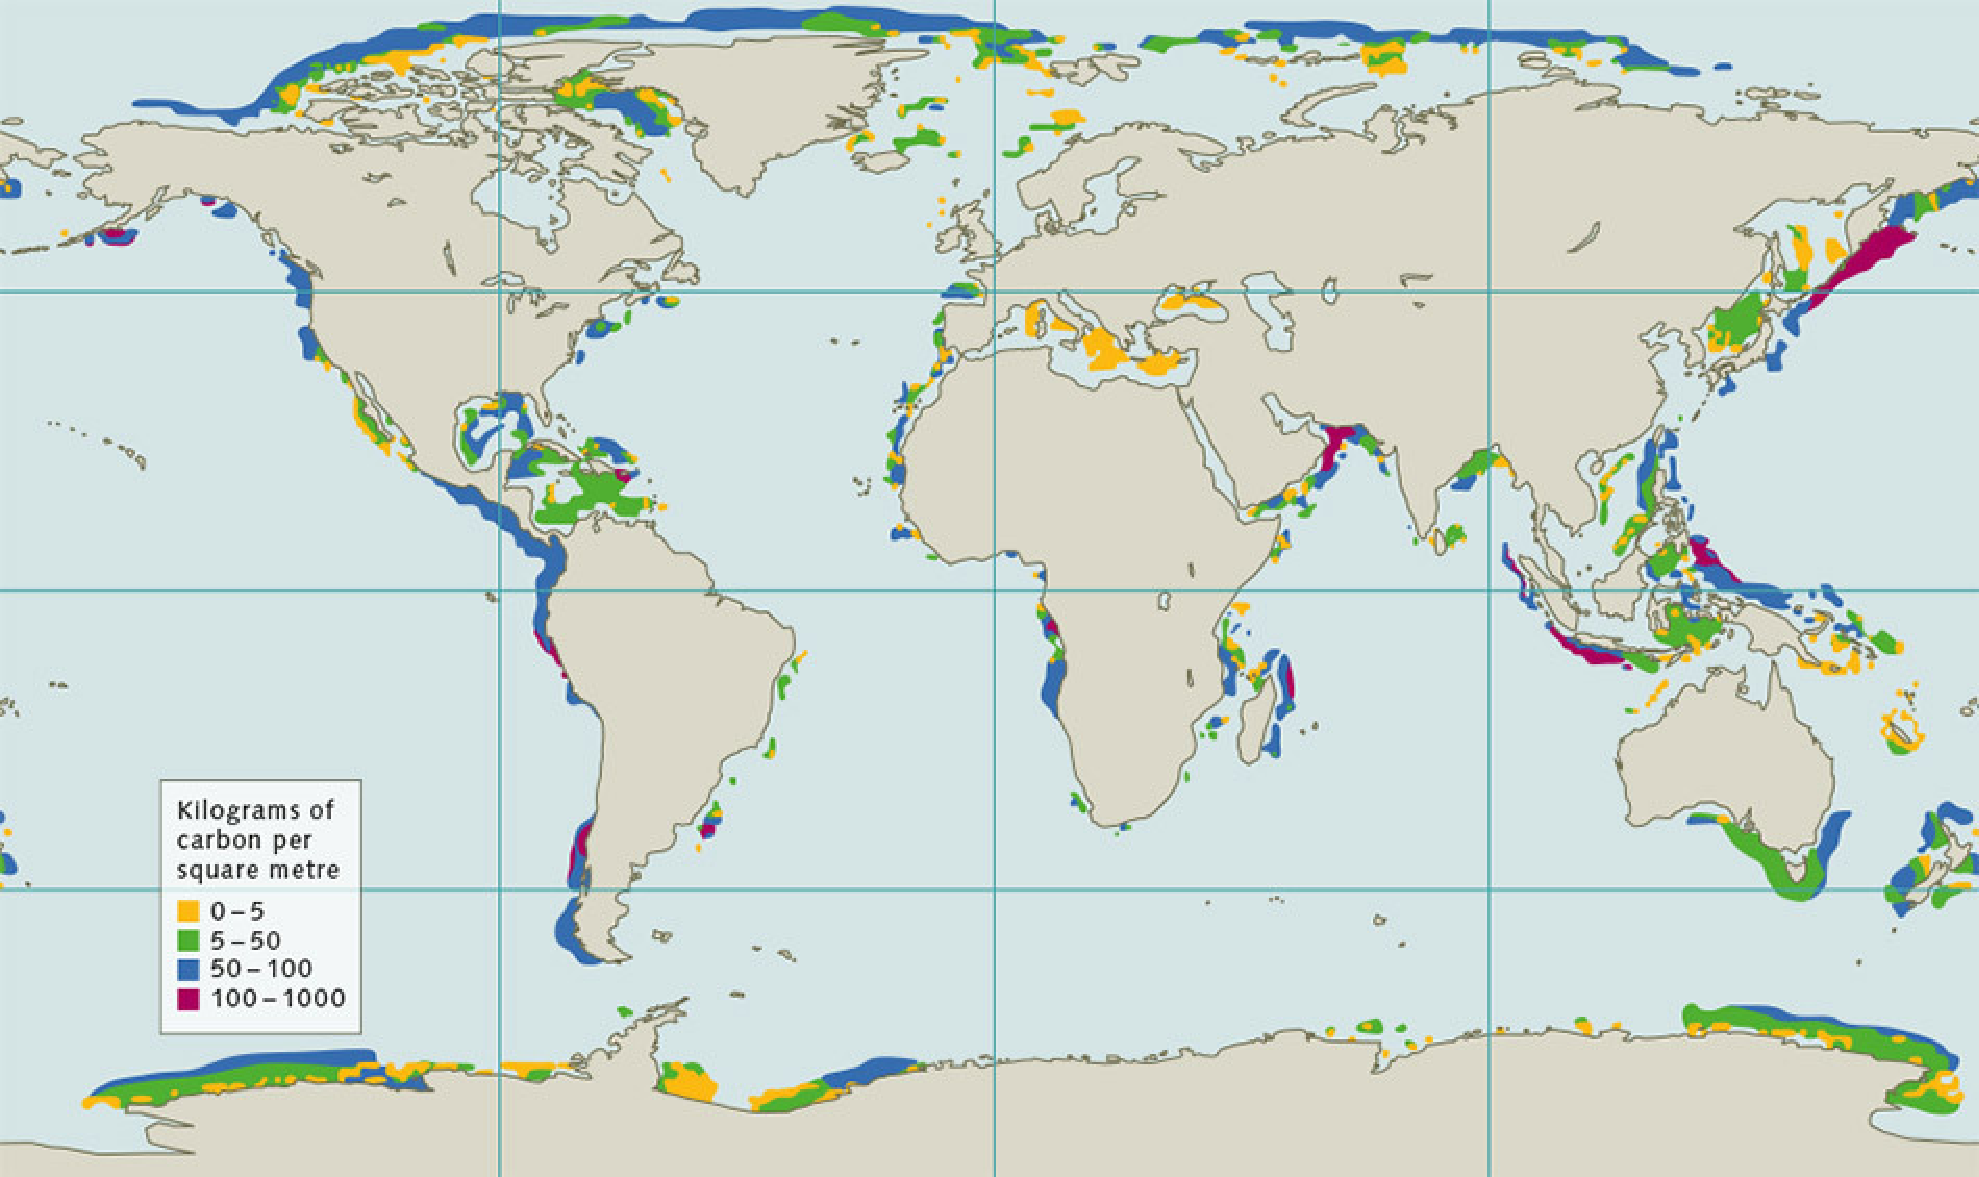
\includegraphics[width=\textwidth]{../pictures/hydrate_map_nice.pdf}
\caption{Estimated methane hydrate occurrences in the world. This map is taken from the World Ocean Review \cite{Bucker2014}, and shows the data of \citet{Wallmann2012}.}
\label{fig:hydrate_map}
\end{figure}

\begin{figure}
\centering
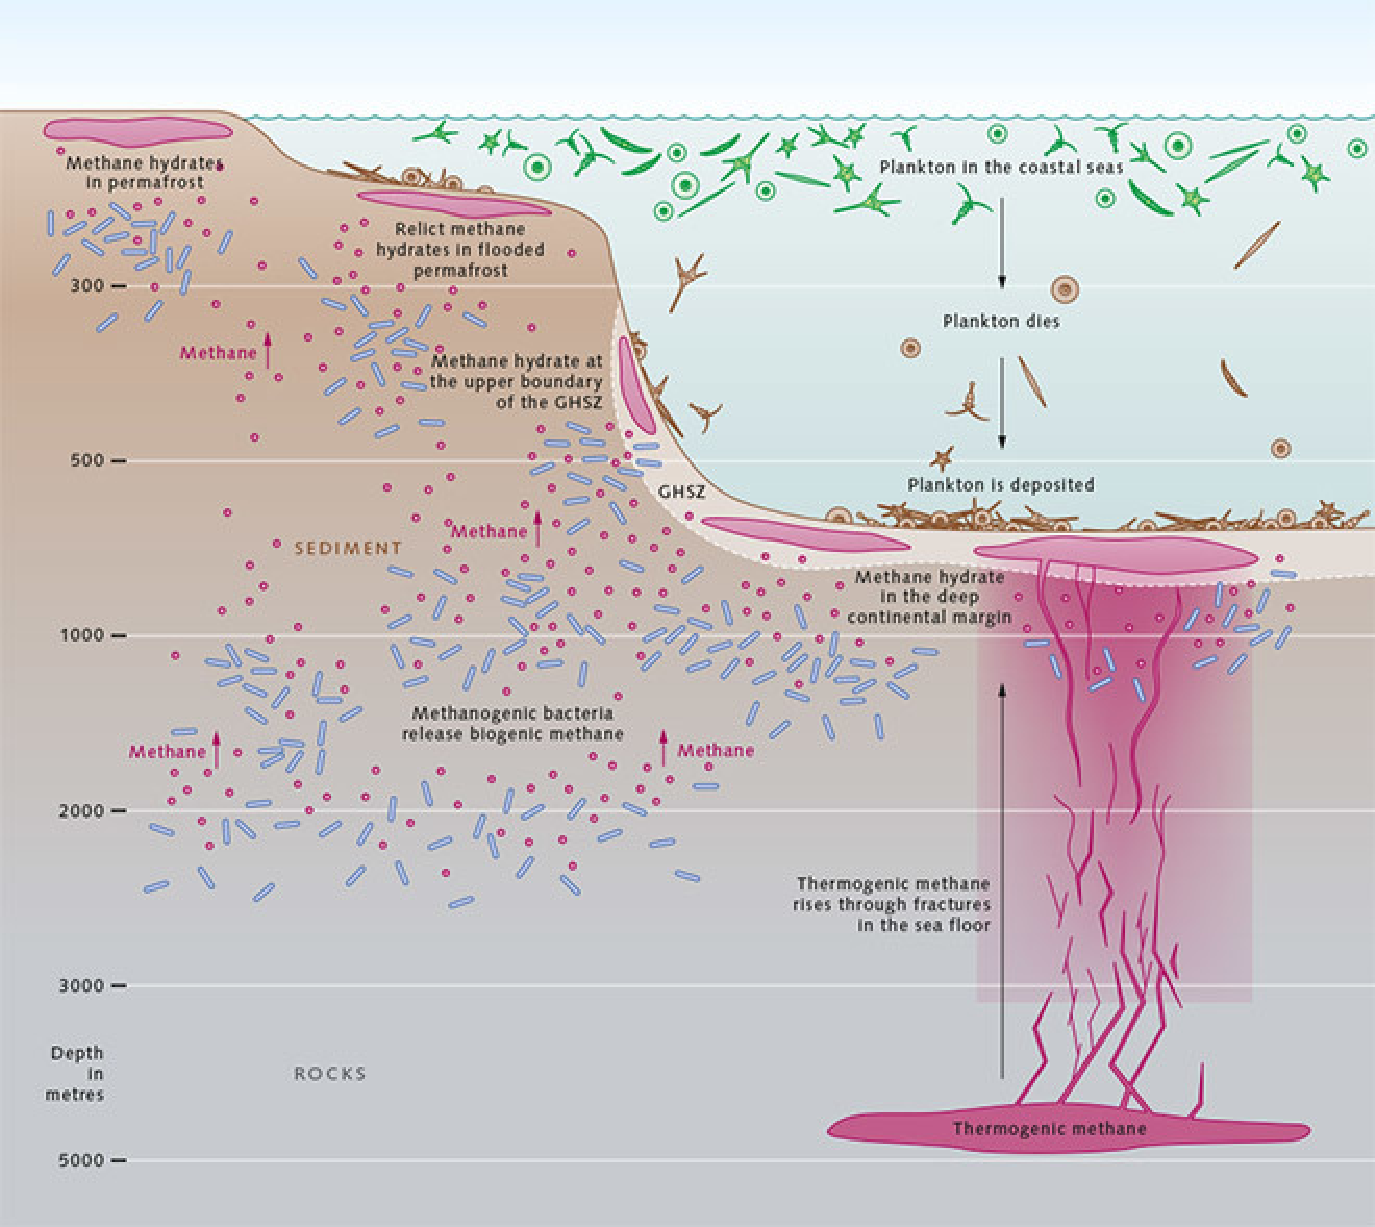
\includegraphics[width=0.8\textwidth]{../pictures/geological_setting.pdf}
\caption{Geological setting of methane hydrate formation. This figure is taken from the World Ocean Review \cite{Bucker2014}.}
\label{fig:geological_setting}
\end{figure}

There are serious risks that must be accounted for if large-scale extraction of methane from hydrates is going to happen. It has for instance been suggested that methane hydrate dissociation can destabilize marine sediments, possibly resulting in underwater landslides \cite{Sultan2004379,Xu2006}. Whether such events can be triggered either by global warming from human activities or from trying to extract methane from the hydrate seem to be an open question \cite{Ning2012}.

\section{Molecular structure}
Different hydrate structures form based on the size of the guest molecules. These structures are characterized by what kinds of cages they contain. The cages are described with the notation $x^y$ where $x$ is the number of faces of a certain type, and $y$ describes the type of face by the number of corners on that face of that type. The most common structures for clathrates with one type of guest molecule are the so-called structure I (sI) and structure II (sII). These structures, along with the cages that form them, are illustrated in figure \ref{fig:methane_hydrate_structure}. The sI structure contains $5^{12}$ and $5^{12}6^2$ cages in ratio $1:3$, the sII structure contains $5^{12}$ and $5^{12}6^4$ cages in ratio $2:1$.  

Small guest molecules, such as methane and ethane, usually form sI hydrates if the conditions for hydrate formation are met \cite{Hester2009}. However, that is only certain if the hydrate is either purely methane or purely ethane. For mixtures of methane and ethane forming gas hydrates, either sI or sII can be formed, depending on the relative amounts of methane and ethane \cite{Subramanian20001981}. 

Not all cages need to be occupied by a guest molecule, so a pure methane hydrate sample can, in addition to its cage structure, be characterized by its cage occupancy. It is common to use the hydrate number to describe cage occupancy, which for methane hydrate is
%
\begin{equation}
	\mathrm{CH_4} \cdot n_w \mathrm{H_2O},
\end{equation}
%
where $n_w$ is the hydrate number. For a fully occupied sI hydrate, the hydrate number would be $n_w = 5.75$. Hydrate numbers have been reported both for laboratory grown methane hydrates and for natural occurring ones. Hydrates grown in laboratory have shown high cage occupancy both with excess water and excess methane, although excess methane yield the highest occupancy. \citet{Circone2005} report values within 5.9 to 6.1 for a relatively wide range of growth conditions: Pressures from 1.8 to \SI{9.6}{\mega\pascal} and temperatures from 263 to \SI{287}{\kelvin}. 

\begin{figure}
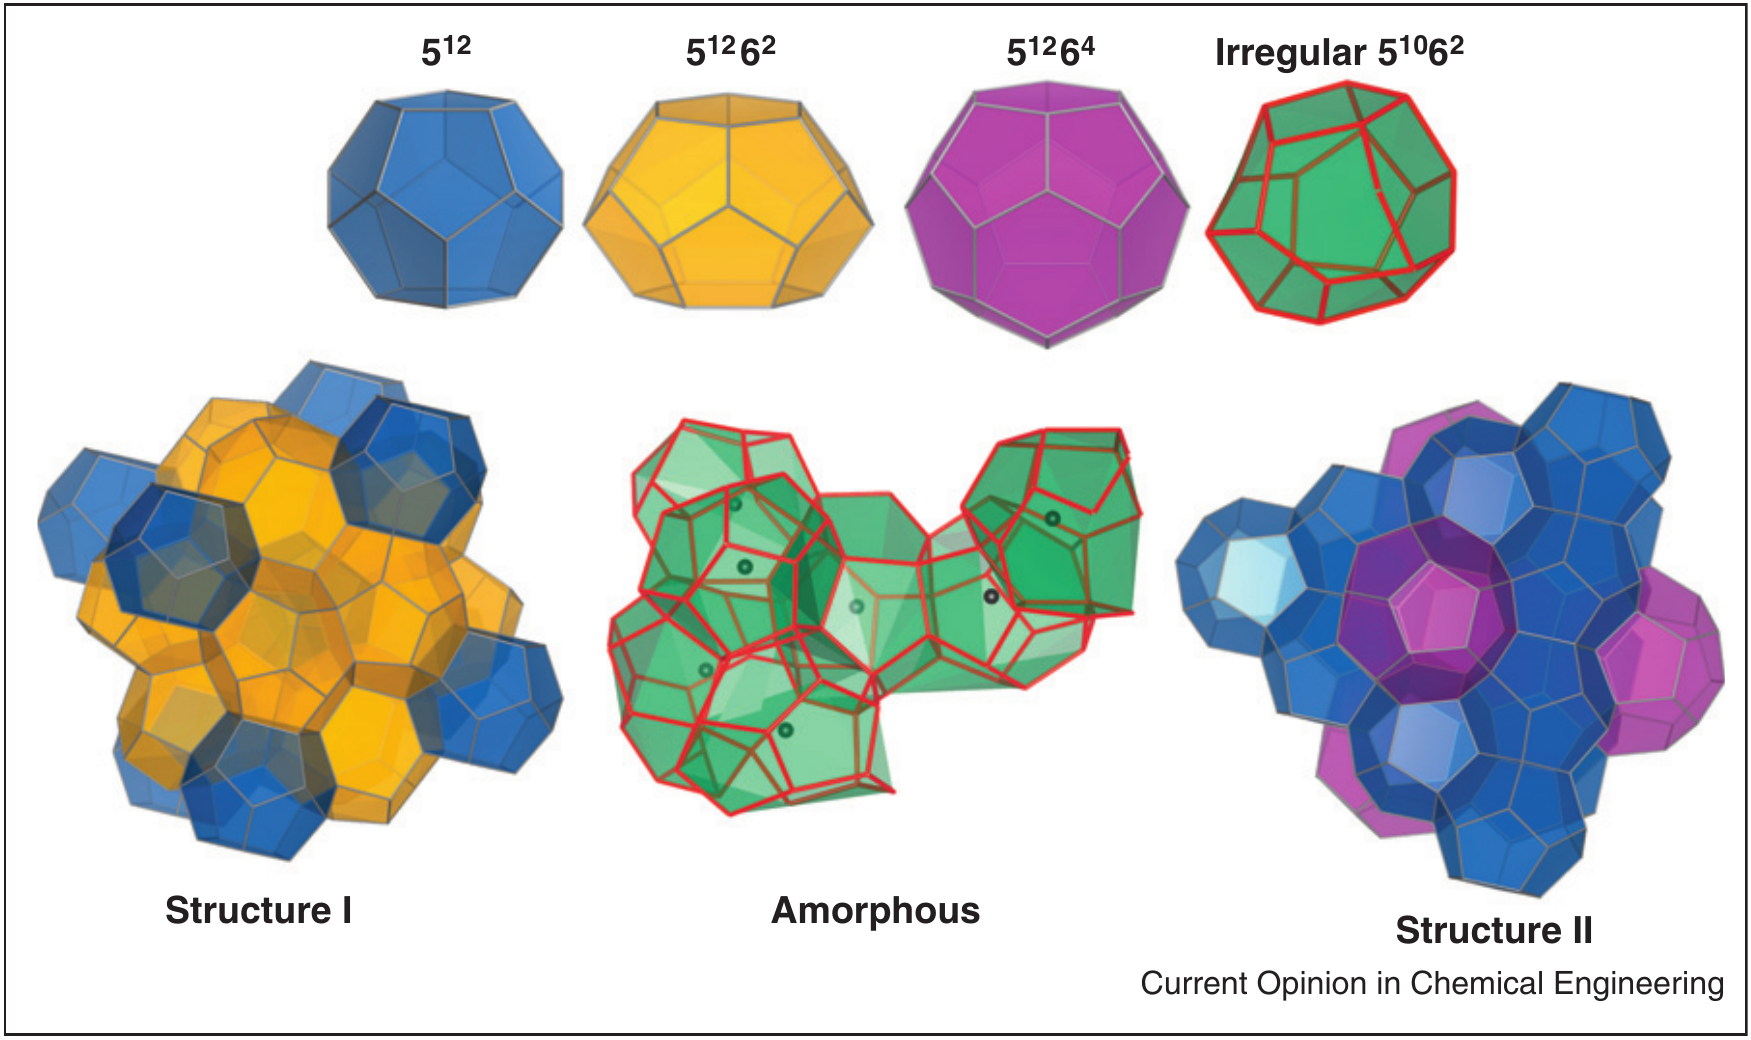
\includegraphics[width=15cm]{../pictures/hydrate_structures.png}
\caption{Cage structures of single guest methane hydrates occurring in nature. Both structure 1 (sI) and structure 2 (sII) contain the $5^{12}$ cage. Reprinted from \citet{Barnes2013} with permission from Elsevier.}
\label{fig:methane_hydrate_structure}
\end{figure}


\section{Mechanical properties from experiments}
An understanding of the mechanical properties of methane hydrates is essential for understanding methane hydrate dissociation processes. Under constant temperature and pressure conditions, the methane hydrate has a higher density than the water + free methane system. Therefore, dissociation of some methane hydrate in a reserve will result in a different stress state of the surrounding hydrate. Also, in a conventional production setting, the hydrate will be drilled, which will impose stresses in the hydrate. 

It turns out that it is hard to say something general about the mechanical properties. In a review paper from 2012, \citet{Ning2012} state:
\begin{quotation}
Few mechanical properties are reported , and their measurements are difficult, partly because it is almost impossible to obtain pure hydrate samples.
\end{quotation}
%
This must be taken into account when going through the experimental results on mechanical properties of methane hydrates. It also means that experimental results probably will not be directly comparable to molecular models of pure samples.

Much of the research has been done on hydrate-bearing sediments, and functional relationships have been proposed that relate the strength of a hydrate-bearing sediment to the pure hydrate strength and the hydrate saturation (the amount of hydrate in the sediment). But since the strength of the mechanical properties of the hydrate are uncertain, the assessment of such relationships is hard. \citet{Ning2012} consider the mechanical properties of pure hydrates essential for understanding the mechanics of hydrate-bearing sediments, which is essential for understanding both how to extract methane and to understand the risks associated with methane extraction from hydrates. Furthermore, almost all strength tests on methane hydrates, tests where the hydrate is subjected to some stress to break it, are axial compression tests, which leaves a limited basis for comparison with simulations. 

\subsection{Typical experimental setup}
A main challenge when doing experiments on methane hydrates is that samples of methane hydrate are not stable in room temperature and atmospheric pressure. Therefore, experimental equipment for the study of mechanical properties of hydrates consist of two main parts: A hydrate formation unit, and a measurement unit, so that the hydrate doesn't need to be removed from its stability conditions during measurement. Sometimes, the measurement unit is actually an axial compression chamber, so that axial tests can be done. Figure \ref{fig:experimental_setup} shows an experimental setup for measuring elastic wave speeds \cite{Waite2000}.

\begin{figure}
\centering
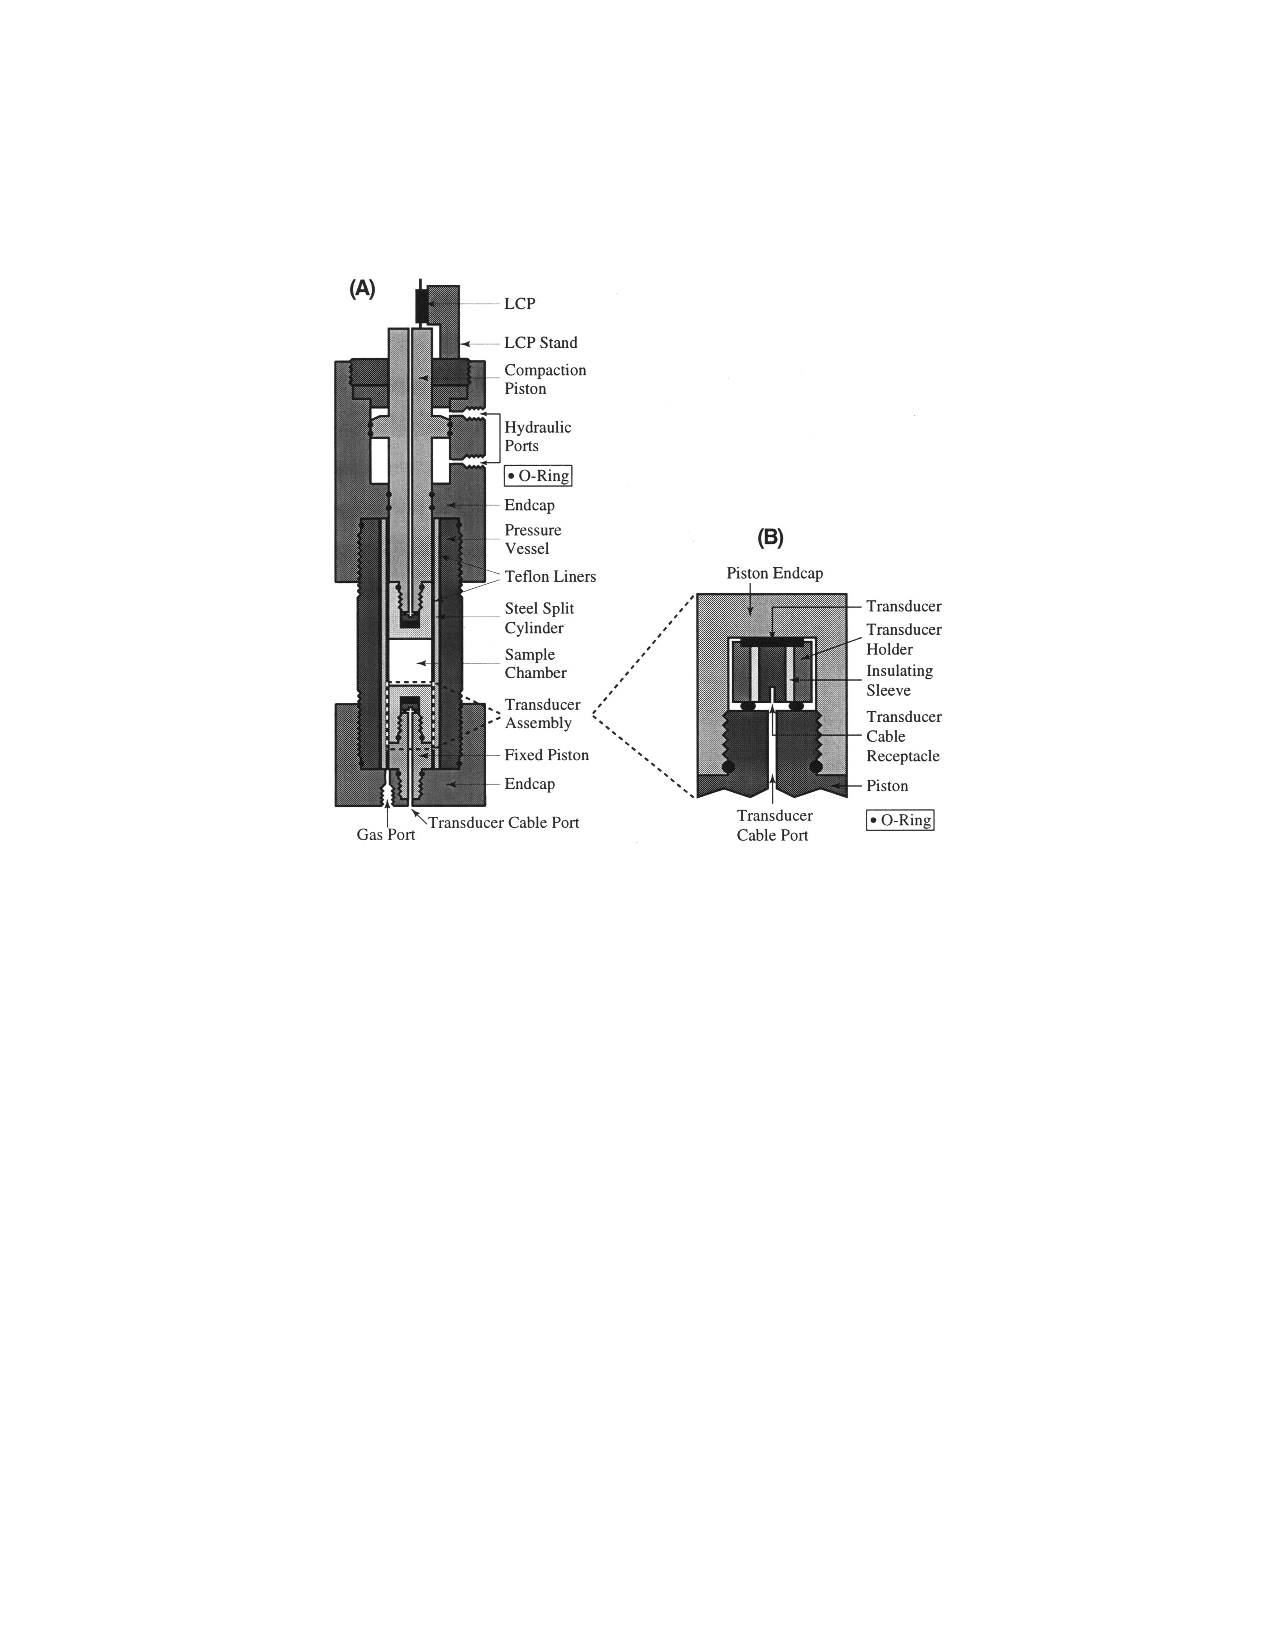
\includegraphics[width=12cm]{../pictures/experimentalsetup.pdf}
\caption{Example of an experimental setup. Reprinted from \citet{Waite2000} with permission from Wiley.}
\label{fig:experimental_setup}
\end{figure}

\subsection{Experimental results}
Even though we cannot guarantee the purity of methane hydrate samples used in experiments, there are still robust findings that are valuable pointers for numerical investigations. \citet{Waite2000} measured mechanical properties using the compressional and shear wave speeds, and assuming the sample to be isotropic and homogeneous. Their results are given in table \ref{tbl:si_mech_exp}.

\begin{table}
\caption{Mechanical properties of sI methane hydrate as reported in \cite{Waite2000}.}
\label{tbl:si_mech_exp}
\centering
\begin{tabular}{c|c}
Property & Value \\
\hline
$V_p$ & \SI{3650\pm 50}{\meter\per\second} \\
$V_s$ & \SI{1890\pm 30}{\meter\per\second} \\
Poisson's ratio & \SI{0.317 \pm 0.006}{} \\
Shear Modulus & \SI{3.2\pm0.1}{\giga\pascal} \\
Isothermal Young's modulus & \SI{7.8\pm 0.3}{\giga\pascal}
\end{tabular}
\end{table}

In the review by \citet{Ning2012}, it is claimed, based on numerous experiments they reviewed, that the tendency for the compressive strength of methane hydrates, is that it increases with increasing confining pressure and decreasing temperature. But it is also stated that all the other mechanical properties depend highly on the temperature, the pressure, the cage occupancy etc., which means results from experiments under slightly different conditions are hard to compare. A surprising observation with regards to compressional strength, is that methane hydrates exhibit strain-hardening for compressional strains as high as around 15-20 \% \cite{Durham2003, Stern1998}, which is very high compared to regular water ice. A strain-hardening curve is shown in figure \ref{fig:strain_hardening}.

\begin{figure}
\centering
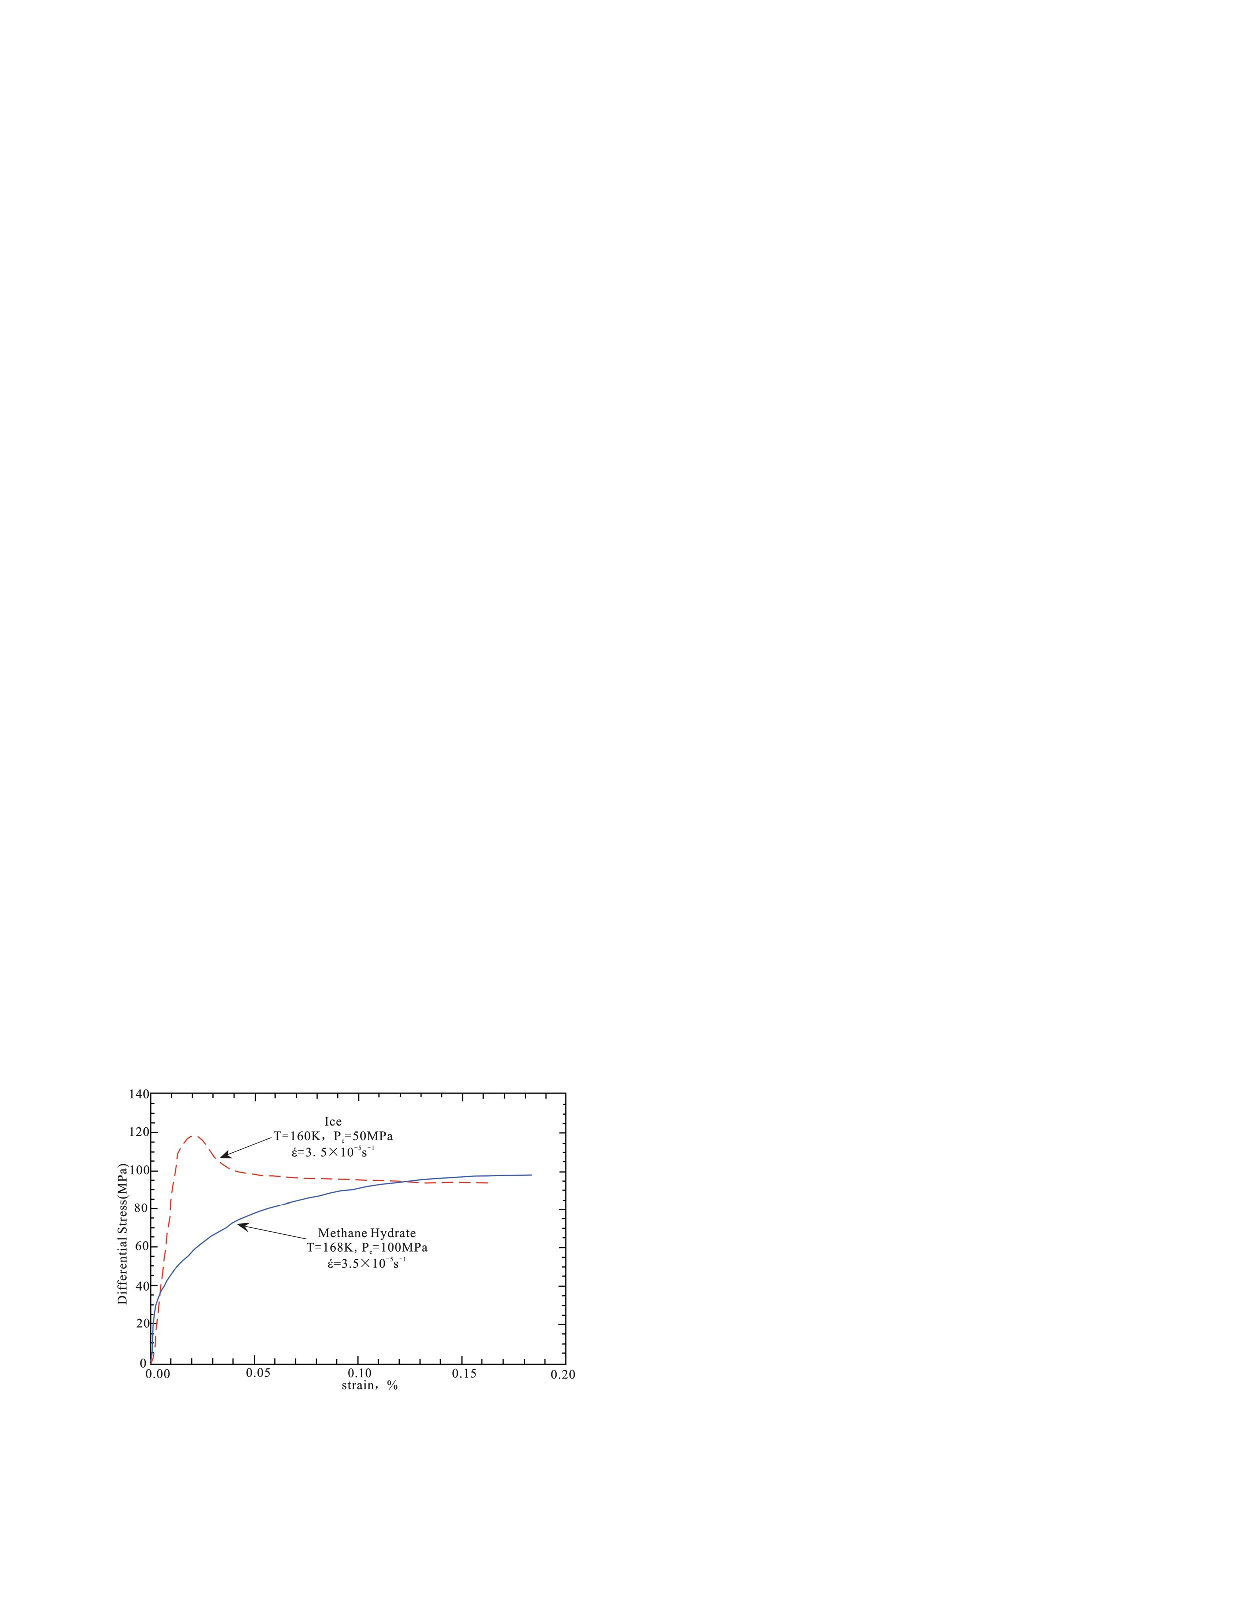
\includegraphics[width=12cm]{../pictures/differential_stress_hydrate.pdf}
\caption{Differential stress–strain curve for methane hydrate and water ice. Note that the axis text on the first axis is wrong. The numbers are not supposed to be in percent, which means the axis range is 0 to 20 \%. Reproduced from \cite{Ning2012} with permission of The Royal Society of Chemistry.}
\label{fig:strain_hardening}
\end{figure}

\section{Classical potential models of water}
Water is a fundamental aspect of life on earth, but it is surprisingly difficult to model all aspects of water within the same modeling framework. Water is difficult to model, and many models are developed in the pursuit of understanding water in all its phases and for various types of systems.

The water molecule can be represented in many different ways, and the most common representation is the ball–stick model of two hydrogen atoms connected to an oxygen atom. In this representation, the parameters for the distance between the oxygen and the hydrogen and the angle between them can been found either experimentally or from quantum mechanics methods such the as the Hartree-Fock method \cite{fock1930naherungsmethode,slater1930note}. Data the the geometry of water is given in table \ref{tb:intro:h2odata}. Another representation of the water molecule is by its wave-function, which can be visualized for example by the electron density around the nuclei of the molecule. Such a representation can be derived from quantum mechanics. Both representations are illustrated in figure \ref{fig:water_molecule}. The quantum mechanic description is too complex to be directly applied in molecular dynamics, so the molecular dynamics representation must be some variation over the connected-particles picture. 

Probably the first to model water using the ball-stick approach was the model of \citet{bernal1933theory} form 1933. The Bernal \& Fowler model is a four-site model where the oxygen and hydrogen nuclei take their positions form the best real-water estimates, but the oxygen-charge is moved slightly along the bisector of the HOH-angle.  This model inspired (and is essentially equal to) the TIP4P model of \citet{Jorgensen1983}, which is one of the most widely studied water models today. Other popular models are the TIP3P model \cite{Jorgensen1983}, a three-particle model where the oxygen charge is placed on the oxygen nucleus, and the SPC water model \cite{berendsen1981interaction}, another three-particle model, where the HOH-angle is optimized for tetrahedral configurations rather that being the correct water molecule configuration. These models come in both flexible and rigid versions, and the rigid versions are often preferred since they reduce the computational cost of simulations. It has also been commented that the hydrogen vibrations are too fast to be treated with classical mechanics \cite{Vega2011}, rendering flexible approaches to the water molecule problematic in non-quantum mechanical models. Both the SPC, TIP3P and TIP4P models are empirically fitted models, which means the models will reproduce some features of water by design. The parameters have gotten better over the years, and \citet{Vega2011} note that the best current parameter set for the TIP4P-model, TIP4P/2005, is probably close to the best possible overall performance of a 4-particle classical potential model of water. To improve the performance, quantum effects must be accounted for in some way. 

\begin{figure}
\begin{minipage}{\textwidth}
\subcaptionbox{The water molecule represented with its individual atoms connected with bonds.}{
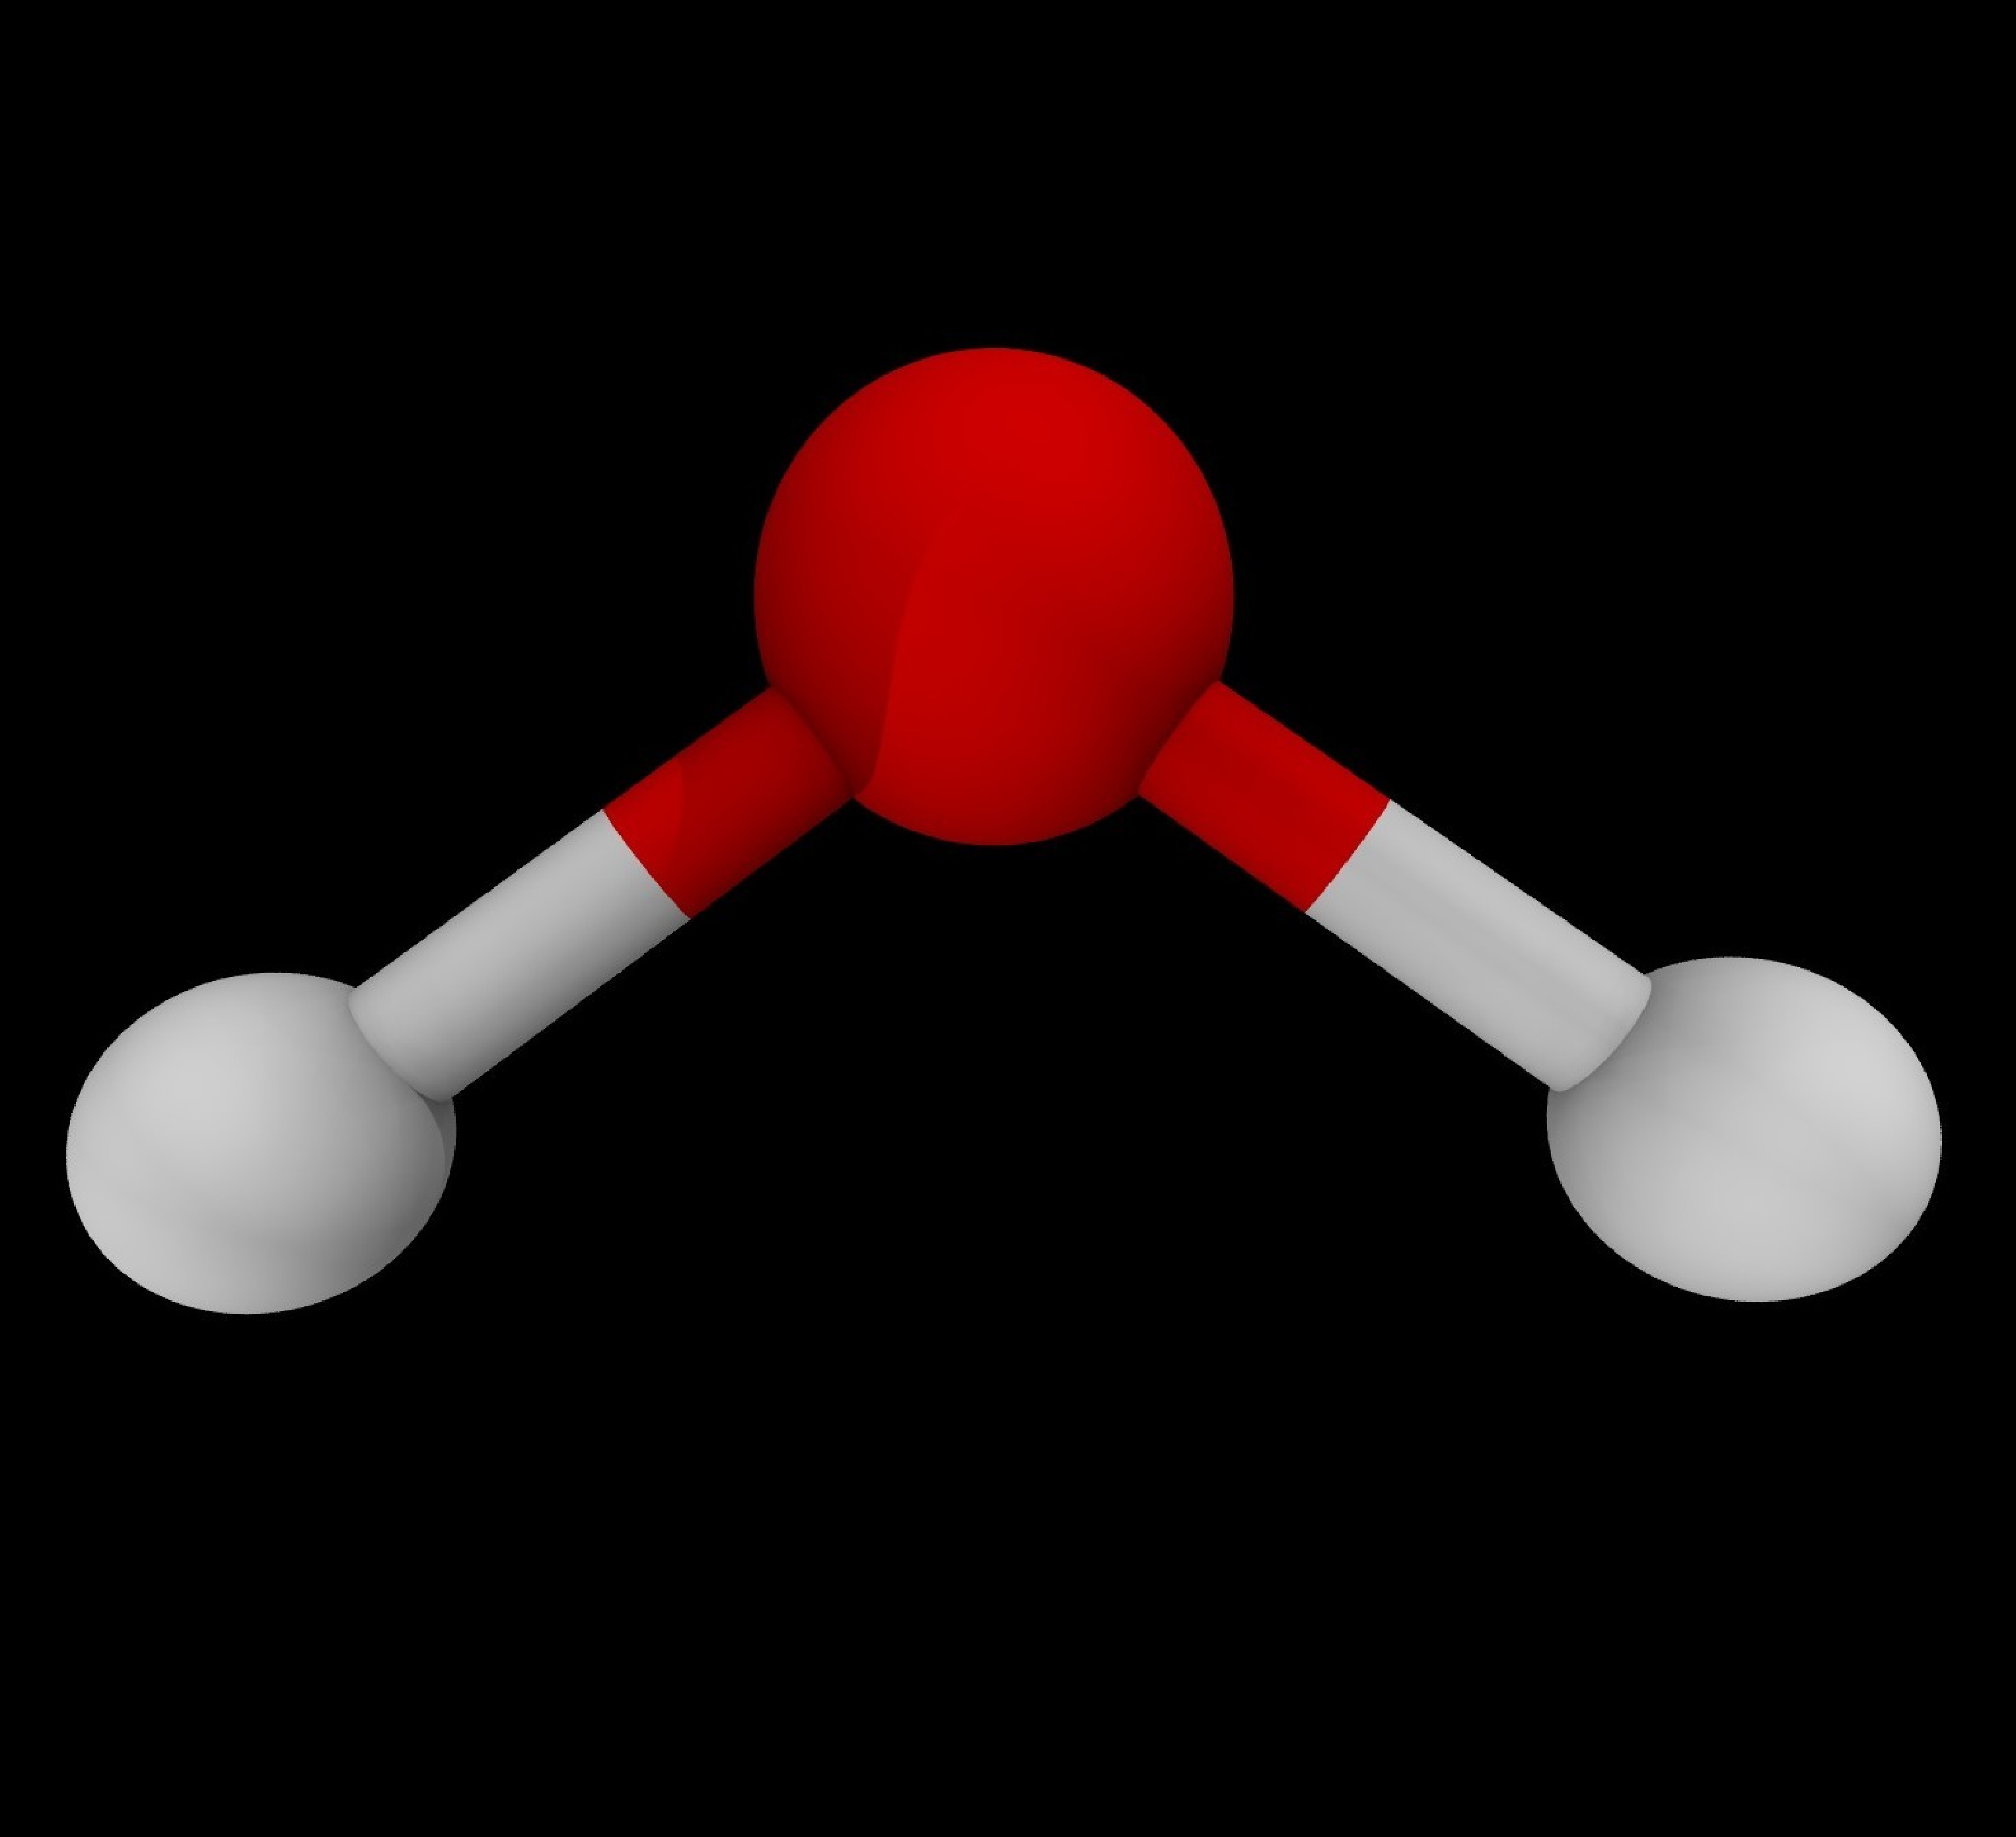
\includegraphics[width=0.52\linewidth]{../pictures/h2o_molecule.pdf}}
\subcaptionbox{Electron density representation of the water molecule. The density is calculated by the Hartree-Fock method. Taken from my simulations for a course at the University of Oslo.}{
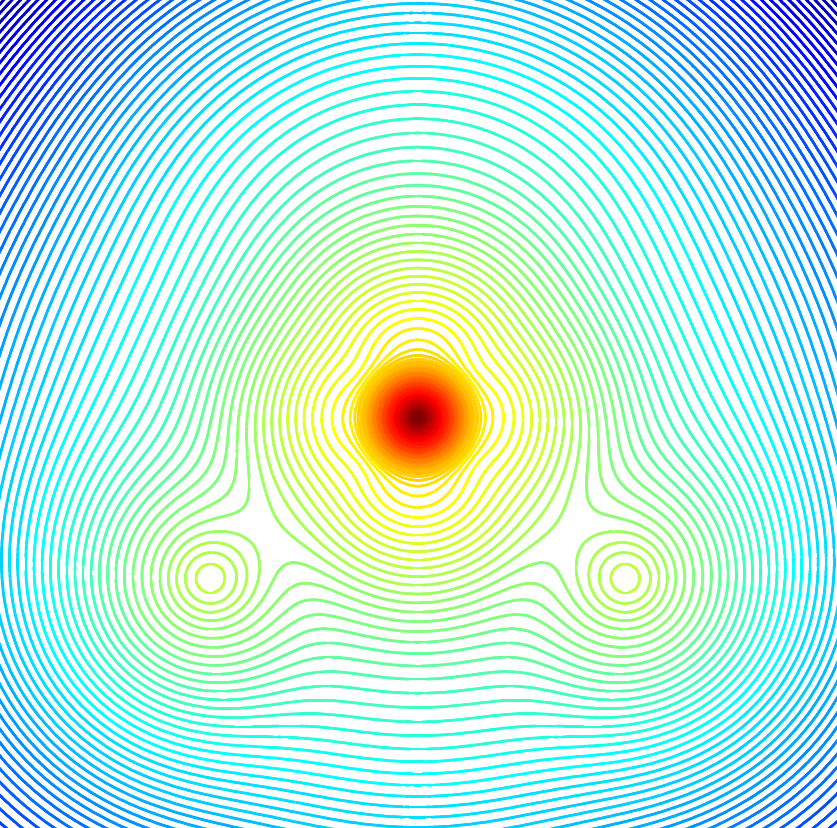
\includegraphics[width=0.48\linewidth]{../pictures/h2o_hf_density.png}}
\end{minipage}
\caption{Two representations of the water molecule.}
\label{fig:water_molecule}
\end{figure}

\begin{table}[h!tb]
\caption{Geometry of the water molecule \cite{Finney2004}.}
\label{tb:intro:h2odata}
\begin{center}
\begin{tabular}{c|c|c}
Description & Symbol & Value \\
\hline
H-O-H angle & $\theta$ & \SI{104.52}{\degree} \\
Distance O-H & $d_{OH}$ & \SI{0.9572}{\angstrom} \\
\end{tabular}
\end{center}
\end{table}

\section{Molecular dynamics modeling of methane hydrates}
Due to the lack of good experimental results, numerical modeling can be important to investigate methane hydrates. One of the ways to model them is through molecular dynamics simulation, where trajectories of individual atoms are calculated using classical equations of motion. 

There are essentially two choices to be made when designing a molecular dynamics simulation: What potential models to use, and what system to simulate. By system, I mean both the initial condition and the conditions during simulation (temperature, pressure, etc.).

For the potential models of methane hydrates, there are two common strategies: All-atom potentials and united-atom potentials. In the all-atom potentials, methane and water are represented by all of its atoms. Interactions between atoms belonging to the same molecule are bonding, and interactions between atoms belonging to different atoms are non-bonding. In the united-atom potentials, all atoms in a molecule are represented by one particle. Interactions between molecules in united atom representations are non-bonding, and the functional form of the potential is usually more complicated than for all-atom models. 

In the first successful simulation of methane hydrate nucleation, \citet{Walsh2009} used a combination of these strategies. The water model was an all-atom model, TIP4P/Ice (described in detail in chapter \ref{ch:models}), and the methane model was a united-atom model, united-atom methane, which is a pure Lennard-Jones potential. Figure \ref{fig:methane_hydrate_growth} shows illustrations of the formation process.  Later, \citet{Jacobson2010b} proposed a coarse-grained model using the united-atom approach both on the water model and the methane model. This model has been used in several studies looking at nucleation and growth of methane hydrates. 

Potentials will be further discussed in chapter \ref{ch:models}.

\begin{figure}
\centering
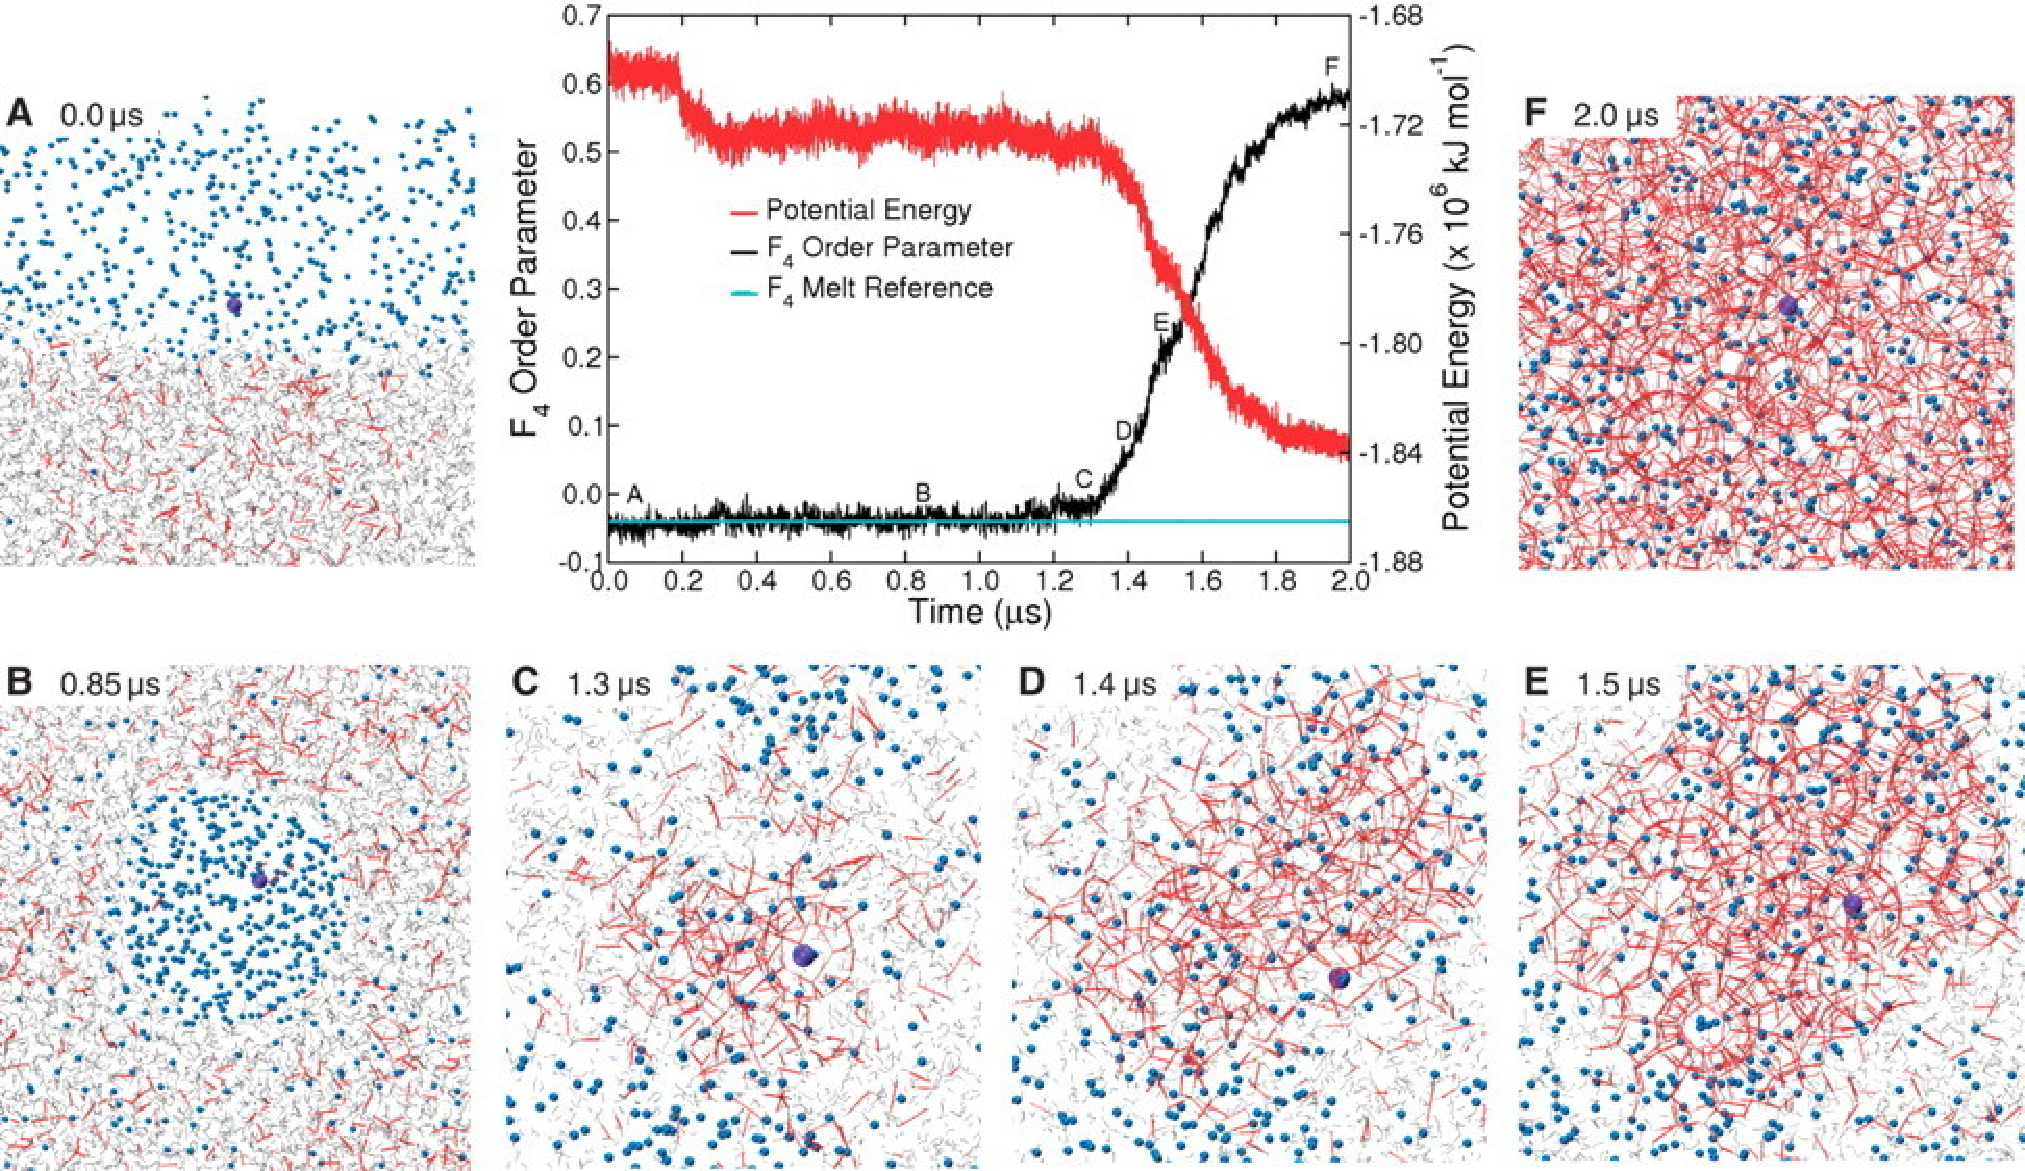
\includegraphics[width=\textwidth]{../pictures/methane_hydrate_growth.pdf}
\caption{Nucleation and growth of methane hydrates. From \citet{Walsh2009}. Reprinted with permission from AAAS.}
\label{fig:methane_hydrate_growth}
\end{figure}

\begin{comment}
\citet{Ning2010} calculate the bulk modulus of sI methane hydrates using several water models and methane models.

\citet{English2015} review molecular modeling of methane hydrates. I will summarize two things they mention: Dissociation and molecular-simulation approaches. They don't cite anyone studying it in conjunction with fracture. 

Chill+ identification of clathrate cages \citet{Nguyen}.
\end{comment}


\section{Quantum mechanical calculations on methane hydrates}
The properties of the sI hydrate cage have been calculated using DFT-analysis. The results differ quite a lot from the experimental values, but since the experimental values are uncertain, it is hard to assess the value of the DFT-analysis.

There have also been some efforts on fitting a methane-water potentials using ab initio quantum mechanical methods. A popular method is by second order Møller--Plesset perturbation theory (MP2). \citet{Anderson2004} used this to develop a potential for argon--water and methane--water interactions and applied the methane--water results on methane hydrates. They fix the internal configuration of each molecule, i.e. the hydrogen positions relative to the oxygen in water and the hydrogen positions relative to carbon in methane. Then they map the six-dimensional energy surface of the methane--water interaction. The dimensions are the C--O distance and five angles describing the relative rotations of the molecules. One of the conclusions is that the Exponential--6-potential better represents the H$_4$\tb{C}--\tb{O}H$_2$ interaction than the Lennard--Jones potential. That study does not cover the interactions between particles of the same species (e.g. water--water).


\section{Molecular dynamics modeling of fracture}
Significant work has been invested to characterize the fracture of relatively simple crystal lattices such as the FCC-lattice. \citet{Abraham19971595} studied fracture in two-dimensional notched solids using the Lennard-Jones potential to model brittle material and the EAM potential \cite{PhysRevB.29.6443} to model ductile material. They do this to investigate general features of a large class of fracture problems, rather than studying properties of a specific substance. Specifically, they observe that the crack tip in brittle fracture becomes unstable when the crack tip speed ($v_c$) reaches around a third of the Rayleigh wave speed ($v_R$). This is somewhat similar to observations of \citet{PhysRevLett.76.2318} from two-dimensional simulations; that the crack must reach a speed of more than one third of the Rayleigh speed to be able to branch. Later, they also studied ductile fracture, and observed characteristic \emph{dislocation loops} near the crack tip. \citet{PhysRevLett.80.746} studied brittle failure of silicon using the potential of \citet{Stillinger1985}. \citet[ch. 6]{doi:10.1142/9789812773326_0001} reviews dynamical fracture of homogeneous lattices, and adds to the observation by Abraham (instability for $v_c > 1/3 v_R$) that the instability velocity depends not only on the Rayleigh wave speed, but also on hyper-elastic (non-linear elastic) properties of the material. Regarding the crack surface; stable, low speed cracks produce mirror interfaces, whereas unstable cracks form either mist (flat but rough) or hackle regions (rough) on the crack surface. In the studies cited in \citet[ch. 6]{doi:10.1142/9789812773326_0001}, tensile strain is applied on the boundary by forcing the position of the atoms in the edge planes parallel to the crack plane. 

\citet{Hantal2014} studied the fracture toughness of illite using clayFF and reaxFF. The actual fracture propagation was not studied -- only the fracture toughness and the stress--strain curves. In that study, the tensile strain was applied in discrete steps by expanding the simulation box normal to the crack plane and remapping all particle positions.

I have not been able to find any studies on molecular dynamics simulations of fracture in methane hydrates.


\section{Research questions}
\label{sec:research_questions}
Since I have not been able to find any studies on fracture of methane hydrates using molecular dynamics, the expectations of what can be done during a master project are limited. Below, I name a few questions concerning methane hydrates that seem within reach to address:

\begin{enumerate}
\item What is the fracture toughness of methane hydrates in simulations? This question is not only interesting to compare with experiments, but to complement experiments. Fracture toughness of materials are usually estimated with standardized mechanical tests, but since such tests are hard to perform on methane hydrates, it is possible that simulation results can complement experimental results, and be important for instance as the pure-hydrate strength going into calculations of the strength of hydrate-bearing sediments. 
\item Is pure methane hydrate ductile or brittle, and is the brittle- or ductileness dependent on the strain rate the sample is subjected to?
\item What does the fracture surface look like? Is it mirror-like or hackle-like? Does the fracture surface develop in time after fracture propagation?
\item How much methane hydrate is dissociated during fracture? How much methane is freed?
\item How predictable are the fracture properties of methane hydrates predictable? Is it such that for a given stress or strain applied to a piece of methane hydrate, the critical stress/strain or the time it takes before it starts cracking can be accurately estimated? Or is it a statistical processes with a wide waiting-time distribution that govern the fracture initiation -- or even propagation?
\item Compressional strain hardening up to almost 20 \% strain. How can this be explained?
\end{enumerate}
Based on these questions, I will produce novel results and insights on molecular dynamics modeling of methane hydrate fractures. Question 1 and 2 will be answered quite conclusively (but only within the model I choose). Question 3 will be discussed along with question 4, offering some descriptive results but little insight. Question 5 results in a claim that I hope to be able to verify in the future. Question 5 will be ignored.

There are also questions regarding how to model methane hydrates, and event within molecular dynamics modeling of methane hydrates, little is actually known -- especially when it comes to fracture. 

\begin{enumerate}
\item What potential best reproduce fracture of methane hydrates?
\item How may cracks be triggered in simulation if the results are going to say something about reality?
\end{enumerate}
These two questions are listed mostly for completeness, as this work is not about potentials itself. However, understanding the limitations of the potentials is essential when doing molecular dynamics, and I also have to choose a potential. Question 2 will be touched, especially with regards to the limitations of molecular dynamics simulations. 
